%--------------------------------------------------------------------------------------------------
% 
\chapter{Knowledge Acquisition Approach}
%--------------------------------------------------------------------------------------------------

This chapter introduces the terms, defines formal structure and steps that form our proposed KA approach. First it introduces the general architecture and steps involved in the process(\hl{ref to chapter}). In the second part, it formalizes the upper ontology and logical constructs required for the KA approach (\hl{ref to chapter}). After that, each of the crucial steps is described in more detail through examples and additions to the base logical structure defined earlier.

\section{Architecture}

In this section we present the general architecture and workflow of the proposed system depicted also on \ref{fig:Architecture}, where arrows represent the workflow, squared boxes separate logical sub-systems and different colors representing functionality groups (see the figure legend).

We can see that the system and its user interaction loop are built around the knowledge base in the center (marked in purple and letter A in Figure \ref{fig:Architecture}). Around the KB, is an integrated Inference engine that can perform inference over the knowledge from the KB. This is represented with the red color and letter B. Tightly connected to the knowledge base and inference engine is a crowdsourcing module, which adds and removes knowledge from the KB based on its consistency among multiple users (Green color and letter F). At the entry and exit point of the systems workflow, there are natural language/logic converters, which are used for communication with the users (blue letter E). Besides the NL endpoints, the system also have a functional endpoint and support, which is used to be able to bring in additional language independent states, such as locations, structured knowledge, etc. In addition to this, the functional part of the application also brings in additional machine learning algorithms and support, and also serves as a glue for all the components, taking care of the interaction between submodules (represented with orange color and letter D). All the modules are triggered either through context (also internal like timer), when it changes, which then causes system to send a request to the user, or through user request directly. This is represented with the arrows, where the blue arrows represent natural language interaction and the orange one structured or functional interaction, where the phone part of the system is interacting automatically without direct user involvement.

\subsection{Knowledge Base}
Internally KB has three components. The main part, which should in any real implementation of the system also be the biggest, is the common-sense knowledge and its upper ontology over which we operate. This part of the system contributes the most to the ability to check the answers for consistency. The more knowledge already exists, the easier becomes to assess the answers. The second part is the user Context KB, which stores the contextual knowledge about the user. This covers the knowledge that the user has provided about himself (section 4.4.2) and the knowledge obtained by mining raw mobile sensors (section 4.4.1). This is represented as the orange arrow, pointing into the context part of the KB. The sensor based context allows the system to proactively target the right users at the right time and thus improve the efficiency and accuracy and also stickiness of the KA process.
The third KB part, is the meta-knowledge and KA rules that drive the dialog and knowledge acquisition process (section 4.3.3). Although in our implementation we used Cyc KB and tested Umko KB, the approach is not fixed to any particular knowledge base. But it needs to be expressive enough to be able to cover the intended knowledge acquisition tasks and meta-knowledge needed for the system?s internal workings. 
After the KB, the second most important part of the architecture is an inference engine (in Fig. 2 marked in red and letter B), which is tightly connected to the knowledge base.  The inference engine needs to be able to operate with the concepts, assertions and rules from the KB and should also be capable of meta-reasoning about the knowledge base?s internal knowledge structures. As the individual components (indicated with red color in Fig. 2) suggest, the inference engine is used for:
?	Checking the consistency of the users? answers (e.g., can you order a car in a restaurant if it?s not food?). 
?	Placement of new knowledge inside the KB.
?	Querying the KB to answer possible questions.
?	Using knowledge and meta-rules to produce responses based on the user and her/his context input (similar in function to the scripts in script-based conversational agents).

 \begin{figure}[htb]
	\centering
		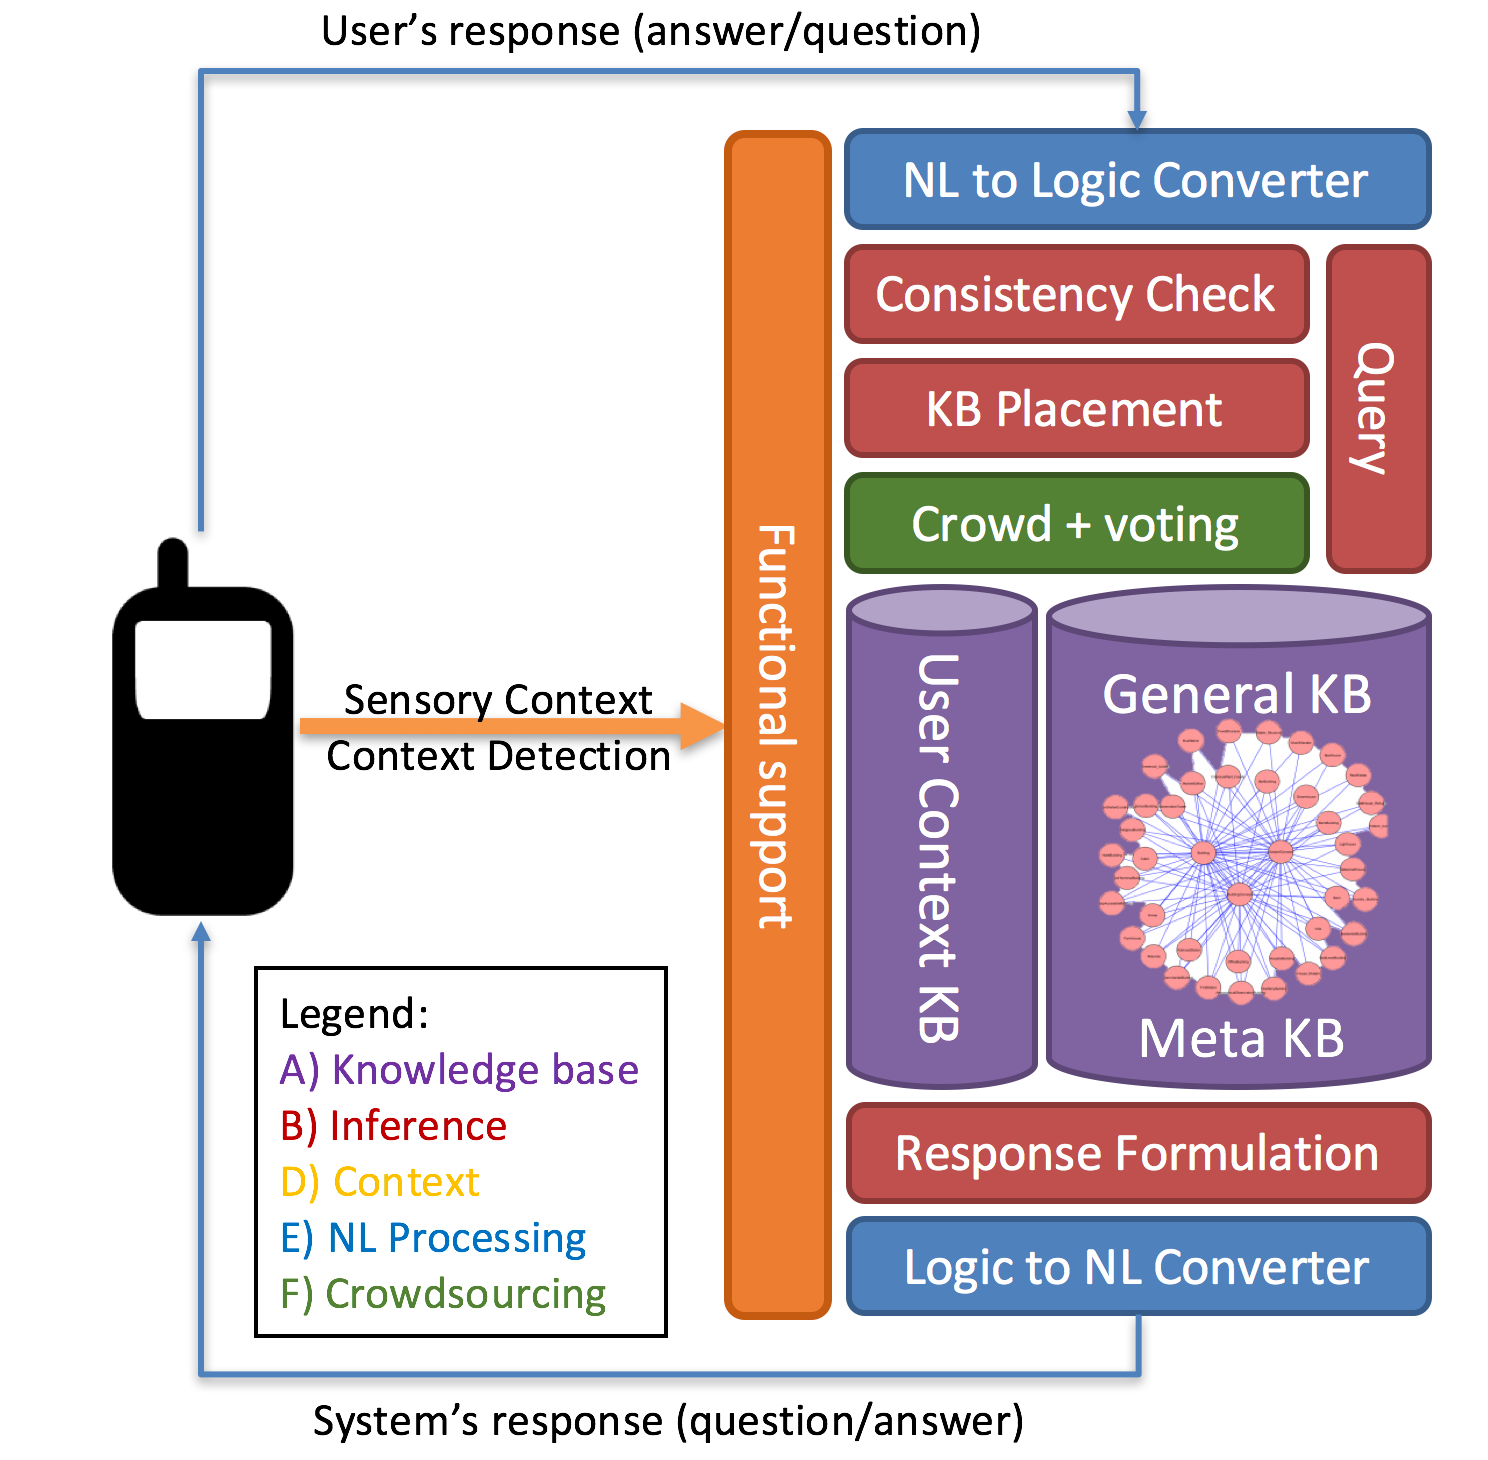
\includegraphics[width=1\textwidth]{figures/architecture.png}
	\caption{General Architecture of the KA system, with a simple interaction loop.}
	\label{fig:Architecture}
\end{figure}

Fig. 2. General Architecture of the KA system, with a simple interaction loop
At both ends of the stacked chain in Fig. 2, there are natural language processing components (marked in blue and with letter E), which are responsible for logic-to-language and language-to-logic conversion (sections 2.4 and 4.5). These are crucial if we want to interact with users in a natural way and thus avoid the need for users to be experts in first order logic. This module and its components are described in more detail in section 4.5.  
Besides the main interaction loop, which implicitly uses crowdsourcing while it interacts with the users, there is an additional component (marked in green and with letter F). This ?crowdsourcing and voting? component handles and decides, which elements of knowledge (logical assertions) can be safely asserted and made ?visible? to all the users and which are questionable and should stay visible only to the authors of the knowledge. If the piece of knowledge is questionable, the system marks it as such and then the question formulation process will check with other users whether it?s true or not. This is described in more detail in section 4.7.
In addition to logic-based components presented above, there is a functional driver system (marked in orange), which glues everything together, forwards the results of inference to the NL converters, accepts and asserts the context into the KB, handles the synchronization between the instances of the systems, etc.
